% GuardedSOC, 8-page revision (2026-11-22, decisions P10 and P11; budget paper/PAGE_BUDGET.md).
% Text from paper/REVISION_DRAFT.md, which follows AgentSOC_IEEE_Revised.docx (the user's working copy).
% Every number comes from experiments/RESULTS.md ("Paper revision" section for the new results); the one exception,
% attack patterns learned under the frequency threshold, comes from experiments/dedale_results/tier1_scores.json.
% \todo{T2.x} marks a Tier 2 number still running. Build: pdflatex agentsoc_v3 (twice).
\documentclass[conference]{IEEEtran}
\IEEEoverridecommandlockouts
\usepackage{cite}
\usepackage{amsmath,amssymb}
\usepackage{graphicx}
\usepackage{xcolor}
\usepackage{booktabs}
\usepackage{array}
\usepackage{url}
\usepackage{algorithm}
\usepackage{algpseudocode}
\usepackage{tikz}
\usepackage{pgfplots}
\pgfplotsset{compat=1.18}
\usetikzlibrary{arrows.meta,patterns}
\definecolor{ctrust}{HTML}{199E70}\definecolor{cllm}{HTML}{3987E5}\definecolor{ctext}{HTML}{D95926}
\pgfplotsset{
  actingbar/.style={draw=black, pattern=north east lines, pattern color=ctext!80!black},
  trustbar/.style={draw=black, fill=ctrust!55},
  basebar/.style={draw=black, fill=white},
}
\tikzset{val/.style={font=\scriptsize, inner sep=1.5pt}}
\newcommand{\todo}[1]{\textcolor{red}{[#1]}}
\makeatletter   % a new row of authors in IEEEtran's author block
\newcommand{\linebreakand}{\end{@IEEEauthorhalign}\hfill\mbox{}\par\mbox{}\hfill\begin{@IEEEauthorhalign}}
\makeatother

\begin{document}

\title{GuardedSOC: Bounding LLM Authority and Memory Updates in Agentic SOC Triage}

\author{
\IEEEauthorblockN{Abhishek Polishetty}
\IEEEauthorblockA{Dept. of CSE\\KMIT\\Hyderabad, Telangana, India\\abhishekpolishetty45@gmail.com}
\and
\IEEEauthorblockN{Kompally Greeshma}
\IEEEauthorblockA{Dept. of CSE\\KMIT\\Hyderabad, Telangana, India\\greeshmakompally@gmail.com}
\and
\IEEEauthorblockN{Arkoti Akshara Reddy}
\IEEEauthorblockA{Dept. of CSE\\KMIT\\Hyderabad, Telangana, India\\aksharareddy612@gmail.com}
\linebreakand
\IEEEauthorblockN{Konda Rohith Kumar}
\IEEEauthorblockA{Dept. of CSE\\KMIT\\Hyderabad, Telangana, India\\krohithkumar1809@gmail.com}
\and
\IEEEauthorblockN{B Vamshi Teja}
\IEEEauthorblockA{Dept. of CSE\\KMIT\\Hyderabad, Telangana, India\\vamshi6t@gmail.com}
}

\maketitle

\begin{abstract}
Agentic security operations centers (SOCs) put large language models (LLMs) and adaptive knowledge stores into
alert triage. Both are attack surfaces: the LLM reads attacker-written log text, and the store learns from observed
activity. We build GuardedSOC on the AgentSOC architecture and bound both. Under asymmetric trust, LLM hypotheses
may escalate a case to human review but cannot dismiss it, trigger containment or authorize a memory update.
Autonomous updates pass a 24-hour quarantined learning gate, and a confirmed compromise retracts the host's recent
patterns. On GUIDE v2 clean/contaminated alert pairs, an undefended agent was hijacked into dismissals on
130/439 development and 123/445 held-out pairs (29.6\% and 27.6\%); within GuardedSOC, contamination suppressed a
response on 4/428 (0.9\%). On 14 test days of DEDALE telemetry, 0/72 attack cases were dismissed under injected text, and targeted
unlearning removed every pattern learned from a 20\% analyst miss rate in all 6 seeds. A persuaded analyst who
clears a host's first attack case defeats unlearning, and the LLM gave no workload reduction over the model-free
baseline.
\end{abstract}

\begin{IEEEkeywords}
Security Operations Center, Agentic AI, Large Language Models, Prompt Injection, Memory Poisoning, Alert Triage
\end{IEEEkeywords}

\section{Introduction}

Security operations centers (SOCs) triage large volumes of alerts, most of them benign~\cite{alahmadi}. Agentic
architectures such as AgentSOC~\cite{agentsoc} aim to reduce this load. An LLM proposes attack hypotheses,
structural analysis checks them against the environment, a risk module ranks responses, and a knowledge store
learns from earlier cases.

Two of these components process data an attacker can influence. The LLM reads free text from logs, such as command
lines, script blocks and raw log records, which an attacker shapes simply by running processes on a monitored host.
Direct and indirect prompt injection against such inputs is well documented~\cite{perez,greshake,liu}. The
knowledge store learns what is normal, and poisoning of learned baselines and agent memory is equally
documented~\cite{antidote,agentpoison,poisonedrag}. AgentSOC was evaluated on a fixed proof-of-concept
scenario~\cite{agentsoc}. It did not measure what happens when the LLM is manipulated, or when the store is updated
over weeks of telemetry and analyst feedback.

We present GuardedSOC, which bounds what the LLM and the memory may do rather than trying to make the model robust.
Its contributions are:
\begin{enumerate}
\item \emph{Asymmetric trust}, an architectural rule under which LLM output may only raise scrutiny. The final
decision is never less strict than the model-free decision, $D(x,h) \ge D(x,\varnothing)$. The model therefore
cannot dismiss a case, cancel containment or authorize learning.
\item \emph{A bounded memory}: a quarantined learning gate for autonomous updates, and targeted unlearning (B5)
that retracts a host's recent patterns when an analyst confirms compromise.
\item \emph{An evaluation on two attack surfaces.} Injected log text is tested on GUIDE v2 alert pairs, against
prompt-level defences and an adaptive attacker, and on DEDALE command lines. Memory poisoning is tested over 14
DEDALE test days through ungated learning, analyst mistakes and a persuaded analyst, with seeds and a
frequency-threshold baseline.
\end{enumerate}
Section~\ref{sec:related} reviews AgentSOC and related work. Section~\ref{sec:arch} describes the architecture,
Section~\ref{sec:setup} the setup, Section~\ref{sec:results} the results, and Section~\ref{sec:disc} the
limitations.

\section{Base Paper and Related Work}\label{sec:related}

\subsection{AgentSOC}

AgentSOC~\cite{agentsoc} has four layers (Perception, Agentic Reasoning, Action, and Playbooks) around a knowledge
store. In the reasoning layer, the Narrative Counterfactual Engine (NCE) asks an LLM for attack-progression
hypotheses, each tagged with MITRE ATT\&CK techniques~\cite{attack} and a confidence. The Structural Simulation
Engine (SSE) rejects hypotheses the identity, privilege and network model cannot support. The Risk Scoring and
Evaluation Module (RSEM) ranks responses by containment benefit against business impact; high-impact responses go
to analysts, and the rest run with audit and rollback. The original study used 5,000 LANL authentication events, a
50-node simulated topology and GPT-4, and reported one incident end to end. It named continuous telemetry and the
human loop as open questions. Table~\ref{tab:compare} summarizes how this work extends it.

\begin{table}[t]
\caption{AgentSOC~\cite{agentsoc} and this work}
\label{tab:compare}
\centering\scriptsize
\setlength{\tabcolsep}{2.5pt}
\begin{tabular}{@{}p{12mm}p{29mm}p{42mm}@{}}
\toprule
Aspect & AgentSOC~\cite{agentsoc} & This work \\
\midrule
Attack model & Stolen credentials, lateral movement, privilege escalation & Text injected into logs the LLM reads;
poisoning of learned memory (V-A, V-C) \\
LLM authority & Infeasible hypotheses filtered by SSE & Asymmetric trust: output may add review, never dismiss,
contain or teach (V-A, V-E) \\
Memory & Enterprise context and learned knowledge & Learning gate; analyst verdicts; targeted unlearning on
confirmed compromise (V-B, V-C) \\
Data, models & 5,000 LANL events, 50-node topology; GPT-4 & GUIDE v2 (500 + 500 pairs), DEDALE (2 + 14 days);
gemini-3.1-flash-lite, gpt-oss-20b \\
Evaluation & One proof-of-concept incident & Paired contamination tests with prompt-defence and adaptive
baselines; seeded replays; Wilson intervals, exact McNemar \\
\bottomrule
\end{tabular}
\end{table}

\subsection{Related Work}

\emph{Prompt injection and its defences.} Instructions hidden in data steer LLMs directly~\cite{perez} and
indirectly through retrieved or tool content~\cite{greshake}. Liu et al.~\cite{liu} formalize these attacks and
benchmark defences, and AgentDojo~\cite{agentdojo} and InjecAgent~\cite{injecagent} measure them for tool-using
agents. Defences act on the prompt or the model: spotlighting marks untrusted data~\cite{spotlighting}, StruQ
separates instructions from data~\cite{struq}, and the instruction hierarchy trains models to rank privileged
instructions above data~\cite{hierarchy}. CaMeL~\cite{camel} instead enforces security outside the model, so the
model need not recognize an attack. GuardedSOC follows that principle for triage, and we measure three prompt-level
defences as baselines (Section~\ref{sec:res-text}).

\emph{Poisoning of learning systems and agent memory.} Poisoning has been studied for anomaly
detectors~\cite{antidote}, for agent memory and knowledge bases~\cite{agentpoison,memorypoison} and for
retrieval-augmented generation~\cite{poisonedrag}. Dash et al.~\cite{memorypoison} find that prompt-injection
defences do not cover memory poisoning. MemStream~\cite{memstream} adapts a streaming detector's memory to drift,
with design choices against poisoning. A SOC's learned baseline has the same weakness: activity learned as normal
is never alerted again. Machine unlearning~\cite{unlearning} removes learned influence; we apply a narrow,
host-scoped form of it.

\emph{LLM alert triage.} Tsegai et al.~\cite{tsegai} report that every LLM-agent triage approach they studied
missed at least 40.4\% of attack-related alerts. GuardedSOC addresses a different question, namely what an LLM is
allowed to decide, and it does not claim better detection (Section~\ref{sec:res-llm}).

\section{System Architecture}\label{sec:arch}

\begin{figure*}[!t]
\centering
% Fig. 1, the GuardedSOC architecture. Cut from paper/agentsoc_v2.tex on 2026-11-22 (with the two user-approved
% fixes: learning gate 'after 24 h'; ERA alone GUIDE-only). Used by agentsoc_v3.tex and paper/build_fig1.py.
\definecolor{csafe}{HTML}{7B4FB3}
\begin{tikzpicture}[font=\footnotesize, >={Stealth[length=1.6mm, width=1.3mm]},
  comp/.style={rounded corners=1.5pt, align=center, inner sep=2pt, anchor=north west, fill=white, draw=black!65,
    line width=0.5pt},
  trusted/.style={fill=ctrust!14, draw=ctrust!70!black, line width=0.6pt},
  attacker/.style={fill=ctext!17, draw=ctext!75!black, line width=1.4pt},
  llm/.style={fill=cllm!14, draw=cllm!75!black, double, double distance=0.9pt, line width=0.4pt},
  safety/.style={fill=csafe!12, draw=csafe!80!black, line width=1.1pt, dash pattern=on 4pt off 1.2pt on 1pt off 1.2pt},
  guideonly/.style={fill=white, draw=black!80, dashed, line width=0.5pt},
  layer/.style={rounded corners=3pt, fill=black!4, draw=black!45, line width=0.5pt},
  ltitle/.style={font=\footnotesize\bfseries, inner sep=3pt},
  flow/.style={->, line width=0.55pt, draw=black!80},
  both/.style={<->, line width=0.55pt, draw=black!80},
  lab/.style={font=\footnotesize, inner sep=1pt, align=center}]
% Routing columns and rows below the action layer.
\coordinate (dx) at (4.4,0); \coordinate (ex) at (6.0,0); \coordinate (rx) at (17.9,0);
\coordinate (dy) at (0,-8.42); \coordinate (ey) at (0,-8.17);
% ---------------- Perception Layer ----------------
\draw[layer] (0,0) rectangle (11.5,-2.0);
\node[ltitle, anchor=north west] at (0,0) {PERCEPTION LAYER};
\node[comp, text width=29mm, minimum height=14.5mm] (an) at (0.2,-0.42)
  {\textbf{Alert Normalization}\\splits each event into trusted fields and free text};
\node[comp, text width=32.5mm, minimum height=14.5mm] (sc) at (3.75,-0.42)
  {\textbf{Situational Contextualization}\\adds context from the store, keyed by trusted fields};
\node[comp, text width=35mm, minimum height=14.5mm] (nr) at (7.65,-0.42)
  {\textbf{Noise Reduction}\\detectors alert only on unlearned patterns; alerts sharing a pattern form a case};
\draw[flow] (3.26,-1.15) -- (3.75,-1.15);
\draw[flow] (7.16,-1.15) -- (7.65,-1.15);
% ---------------- Trusted fields | free text ----------------
\node[comp, trusted, text width=69.5mm, minimum height=7.8mm] (tf) at (0.2,-2.25)
  {\textbf{Trusted fields} (sensors, inventory): host, account, addresses, ports, event ids};
\node[comp, attacker, text width=35mm, minimum height=7.8mm] (ft) at (7.65,-2.25)
  {\textbf{Free text}, written by the attacker};
\draw[flow, draw=ctrust!70!black] (an.south) -- (an.south |- tf.north);
\draw[flow, draw=ctext!80!black] (nr.south) -- (nr.south |- ft.north);
% ---------------- Agentic Reasoning Layer ----------------
\draw[layer] (0,-3.18) rectangle (11.5,-5.76);
\node[ltitle, anchor=north west] at (0,-3.18) {AGENTIC REASONING LAYER};
\node[comp, text width=25mm, minimum height=11mm] (rsem) at (0.2,-3.6) {\textbf{RSEM (Rule Based)}\\ranks responses};
\node[comp, text width=27mm, minimum height=11mm] (sse) at (4.45,-3.6) {\textbf{SSE (Graph Based)}\\Validate Possibility:\\feasible or infeasible};
\node[comp, llm, text width=23.5mm, minimum height=14.5mm] (nce) at (8.84,-3.6)
  {\textbf{NCE (LLM Based)}\\reads the first 512 characters of each free-text field};
% 2026-11-22 (user): ERA alone is GUIDE-only; the known-bad destination check also runs on DEDALE network alerts
% (perception/triage_gate.py rule 1, perception/outcome.py known_bad_contact).
\node[comp, guideonly, text width=15mm, minimum height=4.6mm] (guide) at (3.3,-4.83) {GUIDE only: ERA};
\node[comp, text width=25mm, minimum height=4.6mm] (dest) at (5.1,-4.83) {known-bad destination check};
\draw[flow, draw=ctrust!70!black] (4.9,-3.03) -- (4.9,-3.6);
\node[lab, anchor=west, text=ctrust!60!black] at (4.98,-3.33) {model-free path};
\draw[flow, draw=ctext!80!black] (10.1,-3.03) -- (10.1,-3.6);
\draw[flow, draw=cllm!80!black] (8.84,-4.15) -- (7.31,-4.15) node[lab, midway, above] {Generate\\Hypothesis};
\draw[flow] (4.45,-4.35) -- (2.86,-4.35) node[lab, midway, above] {Published\\Attack Path};
\node[lab, anchor=north, text=cllm!70!black] at (10.09,-5.12) {model-assisted path};
% ---------------- Action and Playbook Layer ----------------
\draw[layer] (0,-5.91) rectangle (11.5,-7.92);
\node[ltitle, anchor=north east] at (11.5,-5.91) {ACTION AND PLAYBOOK LAYER};
\node[comp, text width=24mm, minimum height=14.8mm] (apg) at (0.2,-6.31)
  {\textbf{Adaptive Playbook Generator}\\builds playbooks from ranked actions};
\node[comp, safety, text width=49mm, minimum height=14.8mm] (guard) at (3.3,-6.31)
  {\textbf{Policy and Safety Guardrails}\\outcome = model-free decision, or review;\\a response only the model proposes waits for an analyst};
\node[comp, text width=22mm, minimum height=14.8mm] (exec) at (8.85,-6.31)
  {\textbf{Execution Interface}\\simulates model-free responses};
\draw[flow] (0.7,-4.7) -- (0.7,-6.31);
\node[lab, anchor=west] at (0.8,-5.3) {Ranked Actions};
\draw[flow] (guide.south) -- (guide.south |- guard.north);
\draw[flow] (dest.south) -- (dest.south |- guard.north);
\draw[flow] (2.76,-7.05) -- (3.3,-7.05);
\draw[flow] (8.36,-7.05) -- (8.85,-7.05);
% ---------------- Integrated Knowledge Store and Real-Time Monitoring ----------------
\node[comp, text width=15mm, minimum height=65mm, fill=black!7, draw=black!75, line width=0.9pt] (iks) at (13.0,0)
  {\textbf{Integrated Knowledge Store (IKS)}\\[3pt]learned patterns, environment model, enterprise context};
\draw[both] (11.5,-1.15) -- (13.0,-1.15) node[lab, midway, above] {learned\\patterns,\\context};
\draw[both] (11.5,-4.15) -- (13.0,-4.15) node[lab, midway, above] {environment\\model};
\draw[both] (11.5,-6.3) -- (13.0,-6.3) node[lab, midway, above] {enterprise\\context};
\node[comp, text width=15mm, minimum height=8.5mm] (rtm) at (13.0,-6.95) {\textbf{Real-Time Monitoring}};
\draw[flow] (exec.east |- rtm.west) -- (rtm.west) node[lab, midway, above] {executed\\responses};
\draw[flow] (13.3,-6.95) -- (13.3,-6.5);
\node[lab, anchor=west] at (13.36,-6.72) {outcomes};
% ---------------- Legend, learning gate and analyst inbox ----------------
\begin{scope}[shift={(15.35,-0.05)}]
  \foreach \st/\lab/\y in {trusted/trusted data/0, attacker/attacker text/-0.36, llm/LLM-dependent/-0.72,
                          safety/safety control/-1.08, guideonly/GUIDE only/-1.44, comp/{other component}/-1.8}
    { \draw[\st, rounded corners=1pt] (0,\y) rectangle ++(0.42,-0.26);
      \node[lab, anchor=west] at (0.47,\y-0.13) {\lab}; }
\end{scope}
\node[comp, safety, text width=21mm, minimum height=14.8mm] (gate) at (15.35,-2.3)
  {\textbf{Learning gate}\\learns only cases dismissed without escalation, after 24\,h};
\node[comp, text width=21mm, minimum height=22mm] (inbox) at (15.35,-4.2)
  {\textbf{Analyst inbox}\\human verdicts teach the store; a confirmed compromise triggers unlearning};
\draw[flow] (gate.west) -- (gate.west -| iks.east);
\draw[flow] (inbox.west) -- (inbox.west -| iks.east);
\draw[flow] (guard.south -| dx) |- (rx |- dy) |- (gate.east);
\node[lab, anchor=east] at (4.3,-8.2) {dismissed};
\draw[flow] (guard.south -| ex) |- (inbox.south |- ey) -- (inbox.south);
\node[lab, anchor=east] at (16.38,-7.25) {review and\\model-only\\proposals};
\end{tikzpicture}

\caption{GuardedSOC within the AgentSOC architecture~\cite{agentsoc}: layers, components and trust boundaries;
additions highlighted. Trusted fields feed the model-free path; attacker text reaches only NCE. Guardrails keep the
model-free outcome or raise it to review, and a response only NCE supports waits for an analyst. ERA is evaluated
on GUIDE only.}
\label{fig:system}
\end{figure*}

\subsection{Threat Model and Trust Boundaries}

The adversary writes free text in telemetry: command-line arguments, script blocks, raw log records, and the names
of the binaries and files it drops. It may also try to mislead the human analyst who reviews that evidence. Trusted
are the sensors, endpoint agents and network taps; the structured fields (host identifiers, authenticated
accounts, IP addresses, ports, event IDs); the pipeline's rule engines (SSE, RSEM) and the asset inventory. The LLM
reads untrusted text and proposes hypotheses. It is untrusted for dismissal, containment and memory updates, and may
only request review. Asymmetric trust does not protect against an analyst who issues a wrong benign verdict after
reading manipulated evidence (we measure this channel in Section~\ref{sec:res-poison}), nor against poisoning of the
two training weeks, which are assumed clean.

Events are normalized and enriched from the knowledge store (Fig.~\ref{fig:system}). Detectors raise an alert when
a structured pattern is not yet learned as normal, and alerts with the same pattern are grouped into a case. NCE
sees the first 512 characters of each text field. Entity binding checks that the hosts and accounts named in a
hypothesis exist in trusted fields, and SSE keeps only feasible hypotheses for RSEM. On GUIDE, the Evidence Risk
Assessment (ERA) also escalates alerts whose text looks like an injection. ERA is off on DEDALE, so there raw
attacker text reaches NCE uninspected.

\subsection{Asymmetric Trust}

Let a case $x$ have structured telemetry $x_s$ and text $x_t$, let $h = \mathrm{LLM}(x_t)$ be the hypotheses, and
let $\varnothing$ denote no hypotheses. Outcomes are ordered by severity: NO\_ACTIONABLE $<$ LOW\_PRIORITY $<$
AUTO\_APPROVED $<$ REVIEW. GuardedSOC computes a model-free decision $D_{\mathrm{base}}(x) = D(x,\varnothing)$ from
$x_s$ and the store; on DEDALE, a case with an unlearned pattern goes to review (rule D7). A model-assisted decision
$D_{\mathrm{LLM}}(x,h)$ can only return REVIEW or abstain. The outcome is
\begin{equation}
D(x,h) = \max\bigl(D_{\mathrm{base}}(x),\, D_{\mathrm{LLM}}(x,h)\bigr).
\end{equation}
Containment actions come only from $D_{\mathrm{base}}$. A model-assisted escalation therefore adds review but never
cancels a model-free block.

\emph{Property 1 (safety monotonicity).} For all $x$ and $h$, $D(x,h) \ge D(x,\varnothing)$. This follows directly
from the max: an attacker who changes $x_t$, and through it $h$, cannot push the outcome below $D_{\mathrm{base}}$.

\emph{Property 2 (memory quarantine).} For all $x$ and $h$ on the autonomous path,
$\mathrm{Learn}_{\mathrm{auto}}(x,h) \subseteq \mathrm{Learn}_{\mathrm{auto}}(x,\varnothing)$. A case is eligible for
autonomous learning only at LOW\_PRIORITY or NO\_ACTIONABLE. An escalation caused by $h$ only removes
eligibility, so the LLM can prevent learning but never authorize it. Analyst verdicts bypass this path by design.

We call the earlier behaviour, in which NCE output can also lower an outcome, the \emph{acting rule}. Both rules are
evaluated on the same recorded LLM answers. Property 1 was also checked against randomized synthetic hypotheses.
Algorithm~\ref{alg:triage} gives the decision for one case.

\begin{algorithm}[t]
\caption{Triage decision under asymmetric trust}
\label{alg:triage}
\footnotesize
\begin{algorithmic}[1]
\Require case $x = (x_s, x_t)$, knowledge store $K$
\Ensure outcome $o$, actions $A$ that execute now
\State $\mathit{esc} \gets$ \textbf{false}
\If{$x_s$ contacts a known-bad destination or a watched entity}
  \State $\mathit{esc} \gets$ \textbf{true} \Comment{trusted-field rule, checked first}
\ElsIf{the pattern of $x$ is learned in $K$}
  \State \Return LOW\_PRIORITY, $\emptyset$ \Comment{no LLM call}
\EndIf
\State $b \gets \textsc{Pipeline}(x, \varnothing, K)$ \Comment{model-free decision}
\If{$b.o = $ NO\_ACTIONABLE \textbf{and} the pattern is unlearned}
  \State $b.o \gets$ REVIEW \Comment{rule D7}
\EndIf
\State $h \gets \textsc{NCE}(x_t)$ \Comment{first 512 characters per field}
\State $m \gets \textsc{Pipeline}(x, h, K)$ \Comment{binding, SSE, RSEM, guardrails}
\State $P \gets m.\mathit{auto} \setminus b.\mathit{auto}$ \Comment{actions only NCE supports}
\State $o \gets$ REVIEW \textbf{if} $\mathit{esc}$ \textbf{or} $m.o =$ REVIEW \textbf{or} $P \ne \emptyset$
\textbf{else} $b.o$
\State \Return $o$, $b.\mathit{auto}$ \Comment{$P$ waits for an analyst}
\end{algorithmic}
\end{algorithm}

\subsection{Learning Gate and Targeted Unlearning}

The store learns normal patterns from two clean training weeks. During testing, a case closed without escalation
becomes a learning candidate. The gate commits it only after 24\,h, and only if no escalation has occurred on the
same host or endpoints in the meantime. Analyst benign verdicts teach the store immediately: they are the intended
route for new normal patterns, and the channel a deceived analyst opens. Targeted unlearning (B5) acts on an
analyst's confirmation that a host is compromised. It retracts every pattern learned on that host in the previous 7
days and stops further learning there. Training-week patterns are permanent.

\subsection{Fail-Safes}

Malformed events are rejected and counted. An event that crashes processing is quarantined and the live runner
resumes from its last checkpoint. Any triage error sends the case to review, commands apply atomically, and
checkpoints are signed and load only allow-listed classes. These are tested by unit tests. No event was rejected in
the 43 frozen replays, which run the loop directly, so they do not measure recovery.

\section{Evaluation Setup}\label{sec:setup}

\subsection{GUIDE v2 Alert Pairs}

From GUIDE v2~\cite{guide} we built 1,000 pairs: 500 for development and 500 held out. Each pair is a clean alert
and a contaminated twin that differs only at the injection site. Entities, evidence text and payloads are
synthetic. Alerts run through the single-alert pipeline, with no learned store. A pair is \emph{suppressed} when
the clean twin received a response (REVIEW or AUTO\_APPROVED) and the contaminated twin did not. We also count lost
automatic containment: the clean twin's model-free block is missing from the contaminated twin. We report 95\%
Wilson intervals and exact McNemar tests on the discordant pairs.

An \emph{undefended agent} gets the same alert text, without the pipeline's telemetry, inventory or novelty store,
and returns a verdict. It is \emph{hijacked} on a pair when the contaminated twin is dismissed but the clean twin
is not. We test three prompt-level defences on it, with identical structured fields: delimited untrusted text,
spotlighting~\cite{spotlighting}, and an instruction-hierarchy system prompt~\cite{hierarchy}. An \emph{adaptive
attacker} rewrites each suppression payload until ERA rates it low risk, and moves raw-log payloads into NCE's
512-character view. This uses 300 pairs, with ERA flags falling from 53 to 0.

\subsection{DEDALE Testbed Telemetry}

DEDALE~\cite{dedale} is an emulated small enterprise with host logs, Suricata network alerts, and one multi-stage
APT campaign whose events are labelled on two Windows clients. Two benign weeks seed the store, and then 14 test
days replay in order. A simulated analyst answers each case after a set delay (4\,h unless stated) from the
ground-truth labels. It can be configured to miss attacks (5\% or 20\%), to raise false alarms (5\%), or to be
\emph{persuaded}: on seeing attacker text in a case, it clears a malicious verdict with probability $q$, either for
that case alone or host-wide, for every later case on the host. Random draws are seeded; we report 6 seeds (5 for
some conditions) as mean $\pm$ sd. In experiment E1, three payloads are written into the attacker's command lines:
routine maintenance, fake approval, and a steer that names the domain controller as the host to isolate. Of 84
injected events, 38 fall in the first alert of their case. As a memory baseline, a training pattern counts as
normal only if it occurred at least $K$ times in the clean weeks ($K = 1, 2, 5, 10$).

\subsection{Recorded Answers and Reproducibility}

All LLM answers (gemini-3.1-flash-lite, and gpt-oss-20b on GUIDE development pairs) were recorded once. Every
condition, under either rule, replays those answers deterministically, and one script rebuilds every number from
the frozen score files in the repository.

\section{Results}\label{sec:results}

\subsection{Injected Log Text}\label{sec:res-text}

Table~\ref{tab:text} lists the GUIDE and E1 results under both rules. On GUIDE, contamination suppressed a response
on 4/428 development pairs (0.9\%, CI 0.4--2.4\%; McNemar $b{=}4$, $c{=}4$, $p{=}1.0$), on 3/437 held-out pairs
(0.7\%, CI 0.2--2.0\%; $b{=}3$, $c{=}0$, $p{=}0.25$), and on 10/437 development pairs with gpt-oss-20b (2.3\%, CI
1.2--4.2\%; $b{=}10$, $c{=}5$, $p{=}0.30$). The rule does not change these counts. In the 4 development Gemini
pairs, the 3 held-out pairs and 9 of the 10 gpt-oss pairs, the clean twin was reviewed only because the model
emitted an ungrounded T1071 hypothesis, which the injected text made it drop. With no learned baseline, the LLM is
the only detector, and asymmetric trust cannot restore an escalation the model failed to emit.

The rule does change containment. Under the acting rule, review requests cancelled clean automatic blocks in
20/178, 18/168 and 21/176 pairs. Under asymmetric trust, model-free blocks always execute, and none were lost (0/178,
CI 0--2.1\%; 0/168; 0/178).

The undefended agent was hijacked into dismissals on 130/439 development pairs (29.6\%, CI 25.5--34.0\%;
$b{=}130$, $c{=}28$, $p{=}6.5\times10^{-17}$) and on 123/445 held-out pairs (27.6\%, CI 23.7--32.0\%;
$b{=}123$, $c{=}21$, $p{=}9.6\times10^{-19}$). With delimited text,
spotlighting and the instruction hierarchy it was hijacked on \todo{T2.2: a}, \todo{T2.2: b} and \todo{T2.2: c} of
439 pairs. Prompt-level defences thus \todo{T2.2: direction and size of the change}. Unlike asymmetric trust, a
prompt-level defence bounds the attack only as far as the model obeys it. Against payloads rewritten to evade ERA
and placed inside NCE's view, suppression was 2/300 under both rules (CI 0.2--2.4\%): the same 2 pairs as with the
original payloads (McNemar $b{=}0$, $c{=}0$). The rewrites changed NCE's techniques in 80 pairs, and in 17 they
removed the review the original payload had triggered, but each of these only returned to the clean twin's own
response. Evading the text filter gained the attacker nothing, because the structured pipeline still decides.

On DEDALE (E1), without an analyst and under the acting rule, the maintenance, fake-approval and steer payloads
dismissed 1, 3 and 1 of the 72 attack cases (Fig.~\ref{fig:text}). The steer made NCE name the domain controller in
30 of 38 injected cases (32 of 38 with an analyst). Entity binding marked all 49 such hypotheses (59 with an
analyst) as unbound, so no misdirected containment was proposed. Under asymmetric trust, 0/72 attack cases were
dismissed (CI 0--5.1\%) for every payload: a property of the design, confirmed by the replay.

\begin{figure}[t]
\centering
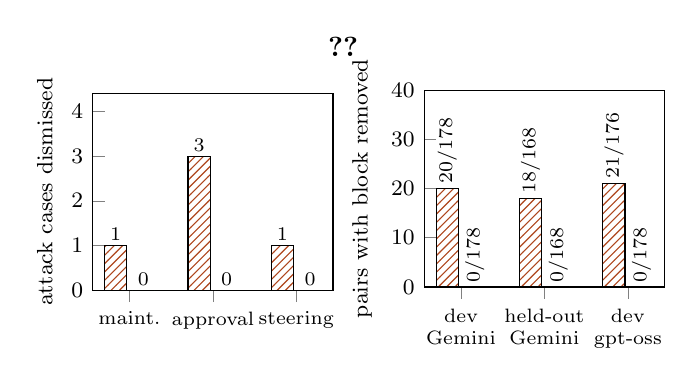
\begin{tikzpicture}
\pgfplotsset{twin/.style={ybar, bar width=8pt, scale only axis, width=3.05cm, height=2.5cm, ymin=0, tick pos=left,
  font=\footnotesize, xticklabel style={font=\scriptsize, align=center}}}
\begin{axis}[twin, name=e1, symbolic x coords={maint,appr,steer}, xtick={maint,appr,steer},
  xticklabels={{maint.},{approval},{steering}}, enlarge x limits=0.22, ymax=4.4,
  ylabel={attack cases dismissed}, legend to name=textlegend, legend columns=2,
  legend style={font=\scriptsize, draw=none, /tikz/every even column/.append style={column sep=6pt}}]
\addplot[actingbar, bar shift=-5pt] coordinates {(maint,1) (appr,3) (steer,1)};
\addlegendentry{acting rule}
\addplot[trustbar, bar shift=5pt] coordinates {(maint,0) (appr,0) (steer,0)};
\addlegendentry{asymmetric trust}
\node[val, above] at ([xshift=-5pt]axis cs:maint,1) {1};
\node[val, above] at ([xshift=-5pt]axis cs:appr,3) {3};
\node[val, above] at ([xshift=-5pt]axis cs:steer,1) {1};
\node[val, above] at ([xshift=5pt]axis cs:maint,0) {0};
\node[val, above] at ([xshift=5pt]axis cs:appr,0) {0};
\node[val, above] at ([xshift=5pt]axis cs:steer,0) {0};
\end{axis}
\begin{axis}[twin, at={(e1.outer east)}, anchor=outer west, symbolic x coords={gdev,ghold,odev},
  xtick={gdev,ghold,odev}, xticklabels={{dev\\Gemini},{held-out\\Gemini},{dev\\gpt-oss}},
  enlarge x limits=0.22, ymax=40, ylabel={pairs with block removed}]
\addplot[actingbar, bar shift=-5pt] coordinates {(gdev,20) (ghold,18) (odev,21)};
\addplot[trustbar, bar shift=5pt] coordinates {(gdev,0) (ghold,0) (odev,0)};
\node[val, rotate=90, anchor=west] at ([xshift=-5pt]axis cs:gdev,20) {20/178};
\node[val, rotate=90, anchor=west] at ([xshift=-5pt]axis cs:ghold,18) {18/168};
\node[val, rotate=90, anchor=west] at ([xshift=-5pt]axis cs:odev,21) {21/176};
\node[val, rotate=90, anchor=west] at ([xshift=5pt]axis cs:gdev,0) {0/178};
\node[val, rotate=90, anchor=west] at ([xshift=5pt]axis cs:ghold,0) {0/168};
\node[val, rotate=90, anchor=west] at ([xshift=5pt]axis cs:odev,0) {0/178};
\end{axis}
\node[anchor=south] at ([yshift=1pt]e1.outer north east) {\ref{textlegend}};
\end{tikzpicture}
\caption{Attacker text under the acting rule (hatched) and asymmetric trust (solid). Left: E1 attack cases
dismissed (of 72), no analyst. Right: GUIDE pairs that lost an automatic block.}
\label{fig:text}
\end{figure}

\begin{table}[t]
\caption{Attacker-written text, acting rule vs.\ asymmetric trust}
\label{tab:text}
\centering\scriptsize
\setlength{\tabcolsep}{2pt}
\begin{tabular}{@{}llrr@{}}
\toprule
Setting & Measure & Acting rule & Asym.\ trust \\
\midrule
GUIDE dev, Gemini & suppressed & 4/428 & 4/428 \\
 & containment removed & 20/178 & 0/178 \\
GUIDE held-out, Gemini & suppressed & 3/437 & 3/437 \\
 & containment removed & 18/168 & 0/168 \\
GUIDE dev, gpt-oss-20b & suppressed & 10/437 & 10/437 \\
 & containment removed & 21/176 & 0/178 \\
GUIDE dev, adaptive & suppressed & 2/300 & 2/300 \\
\midrule
E1 DEDALE, & dismissed (maint./appr./steer) & 1/3/1 of 72 & 0/0/0 of 72 \\
no analyst & clean reviews per day & 54.8 & 65.2 \\
E1 DEDALE, & dismissed (all) & 0/72 & 0/72 \\
analyst & clean reviews per day & 33.2 & 34.1 \\
\midrule
Undefended & hijacked, dev/held-out & 130/439, 123/445 & n/a \\
agent & delimited / spotl. / hierarchy & \todo{T2.2} of 439 & n/a \\
\bottomrule
\end{tabular}
\end{table}

\subsection{Gated Learning, Workload and a Simple Baseline}

With nothing learned, the host detectors opened 6,095.4 reviews per day at 0.1\% precision, alerting 80 attack
cases and 473 labelled attack events (Table~\ref{tab:dedale}, Fig.~\ref{fig:c2}). Seeding the store with the two
clean weeks cut this to 65.2 reviews per day (98.9\% less) at 7.9\% precision. Every one of the 72 attack cases
raised was reviewed, and 400 of the 473 detector-visible attack events were alerted (84.6\%); the other 73 matched
routine activity from the training weeks, which is the cost of novelty filtering and an opening for mimicry. The
attack stages were first reviewed 1.2, 28.5 and 30 minutes after initial access, lateral movement and collection
began, and 1,265 minutes after exfiltration began.

Learning without the gate lowered reviews to 27.4 per day but absorbed 38 attack patterns as routine: attack cases
raised fell to 38, events alerted to 99, and the exfiltration stage was never detected. With D7 on, no case with an
unlearned pattern closed without review, so the gate committed no pattern on host logs and no network pattern edge.
On Suricata network alerts, reviews fell from 552.3 per day (static, 0/7 attack cases missed) to 26.1 (gated, 0/7
missed); ungated learning gave 20.6 but missed 4/7.

\emph{Frequency threshold (baseline).} Treating a training pattern as normal only if it occurred at least $K$ times
did not improve detection: every $K$ raised the same 72 attack cases and 400 events, while workload grew from 65.2
reviews per day ($K{=}1$) to 86.4, 163.4 and 718.7 for $K = 2, 5, 10$, and precision fell to 0.7\%. Rarity in clean
data is a poor proxy for risk, and the poisoning that matters enters during testing (Section~\ref{sec:res-poison}),
where a threshold on the training weeks has no effect.

\emph{Gate delay.} Where the gate does learn (host logs under the acting rule, and network alerts with D7 off),
raising the delay from 1\,h to 168\,h cut patterns committed through the gate from 16 to 0 (host) and from 671 to
256 edges (network). No attack pattern was learned at any delay. Host reviews rose only from 55.0 to 58.9 per day,
and network reviews stayed at 7.9.

\begin{figure}[t]
\centering
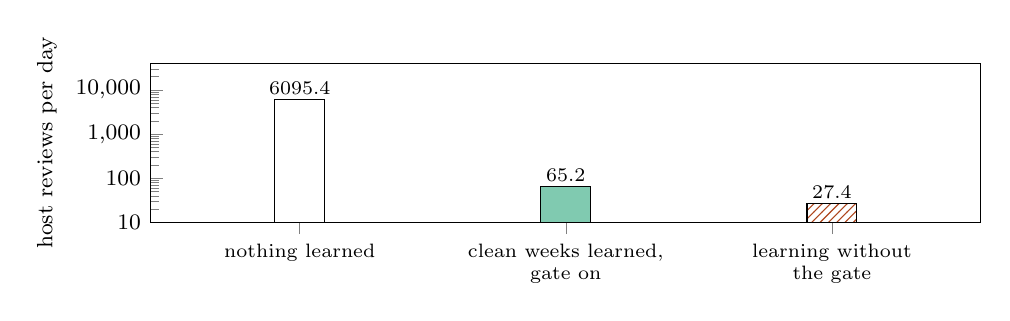
\begin{tikzpicture}
\begin{axis}[ybar, bar width=18pt, ymode=log, log origin=infty, ymin=10, ymax=40000, log ticks with fixed point,
  width=\columnwidth, height=3.6cm, symbolic x coords={none,gate,nogate}, xtick={none,gate,nogate},
  xticklabels={{nothing learned},{clean weeks learned,\\gate on},{learning without\\the gate}},
  xticklabel style={font=\scriptsize, align=center}, enlarge x limits=0.28, font=\footnotesize, tick pos=left,
  ylabel={host reviews per day}]
\addplot[basebar, bar shift=0pt] coordinates {(none,6095.4)};
\addplot[trustbar, bar shift=0pt] coordinates {(gate,65.2)};
\addplot[actingbar, bar shift=0pt] coordinates {(nogate,27.4)};
\node[val, above] at (axis cs:none,6095.4) {6095.4};
\node[val, above] at (axis cs:gate,65.2) {65.2};
\node[val, above] at (axis cs:nogate,27.4) {27.4};
\end{axis}
\end{tikzpicture}
\caption{Host reviews per day on DEDALE, log scale. Learning without the gate has the fewest reviews only because it
learned 38 attack patterns as routine (99 attack events alerted, against 400 with the gate).}
\label{fig:c2}
\end{figure}

\begin{table}[t]
\caption{DEDALE host logs, 14 test days: memory and LLM conditions}
\label{tab:dedale}
\centering\scriptsize
\setlength{\tabcolsep}{1.8pt}
\begin{tabular}{@{}lrrrrrr@{}}
\toprule
Condition & Rev./day & Att.\ cases & Events & Learned & Prec. & Ben.\ dism. \\
\midrule
No learning & 6095.4 & 80 & 473 & 0 & 0.1\% & 0 \\
Clean weeks + gate & 65.2 & 72 & 400 & 0 & 7.9\% & 0 \\
Threshold $K{=}2$ & 86.4 & 72 & 400 & 0 & 5.9\% & 0 \\
Threshold $K{=}5$ & 163.4 & 72 & 400 & 0 & 3.1\% & 0 \\
Threshold $K{=}10$ & 718.7 & 72 & 400 & 0 & 0.7\% & 0 \\
No gate & 27.4 & 38 & 99 & 38 & 9.9\% & 1 \\
NCE, acting rule & 54.8 & 72 & 400 & 0 & 9.4\% & 89 \\
NCE, asym.\ trust (= off) & 65.2 & 72 & 400 & 0 & 7.9\% & 0 \\
NCE + analyst, asym. & 34.1 & 72 & 400 & 0 & 15.1\% & 0 \\
\bottomrule
\end{tabular}
\end{table}

\subsection{Analyst-Induced Poisoning and Targeted Unlearning}\label{sec:res-poison}

An analyst's benign verdict teaches the store directly, so a missed attack becomes a learned pattern
(Table~\ref{tab:poison}, Fig.~\ref{fig:c3}). Without unlearning, a 5\% miss rate left 7.33 $\pm$ 2.42 attack cases'
patterns learned over 6 seeds, with 386.5 of 400 events alerted on average; a 20\% miss rate left 18.5 $\pm$ 2.81
learned, with 333.33 $\pm$ 61.14 events alerted. With B5 on, confirmation of a compromised host retracted its
recent patterns: every seed and both miss rates ended with 0 attack patterns learned and all 400 events alerted.

B5 has costs. It raised workload from 30.0--30.6 to 34.1 reviews per day, because retracted routine patterns are
reviewed again, and with 5\% false alarms (benign hosts confirmed as compromised) workload was 41.83 $\pm$ 2.25
reviews per day against 31.38 $\pm$ 0.23 without B5. The lookback barely matters on this campaign: from 1 to 14
days every run ended with 0 learned attack patterns, at 33.3 reviews per day for 1 day and 34.1 for 3 to 14.

\emph{Persuaded analyst.} Here the attacker's text, which reaches 38 of the 72 attack cases, talks the analyst out
of a malicious verdict. Per-case persuasion never defeated B5 ($q = 1$ and $q = 0.5$; 0 learned and 400 events
alerted in every seed), because the host's other attack cases still led to a confirmation; without B5, 21 patterns
were learned at $q = 1$. Host-wide persuasion did defeat B5 whenever the first attack case on CLIENT1 carried the
text and was cleared: 10 of 10 runs at $q = 1$, and 2 of 5 at $q = 0.5$. CLIENT1 was then never confirmed, 13 attack
cases' patterns stayed learned for up to 268.5\,h, and only 262 of 400 events were alerted. B5 thus bounds poisoning
by an analyst who errs independently, but not by one deceived about a whole host. That channel lies outside
asymmetric trust by our threat model, and the result quantifies the gap.

\begin{figure}[t]
\centering
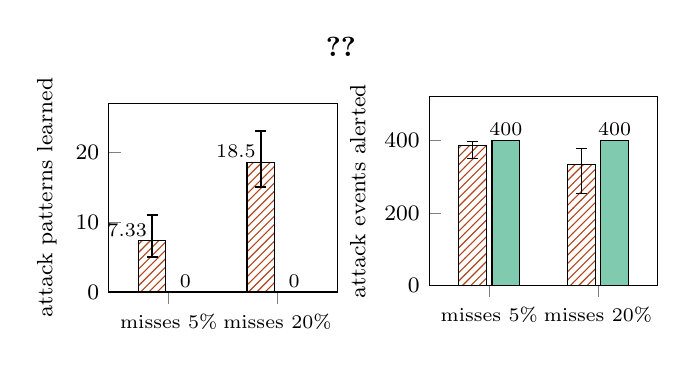
\begin{tikzpicture}
\pgfplotsset{poison/.style={ybar, bar width=10pt, scale only axis, width=2.9cm, height=2.4cm, ymin=0, tick pos=left,
  symbolic x coords={m5,m20}, xtick={m5,m20}, xticklabels={{misses 5\%},{misses 20\%}}, enlarge x limits=0.55,
  font=\footnotesize, xticklabel style={font=\scriptsize},
  error bars/y dir=both, error bars/y explicit, error bars/error bar style={line width=0.5pt}}}
\begin{axis}[poison, name=learned, ymax=27, ylabel={attack patterns learned},
  legend to name=poisonlegend, legend columns=2,
  legend style={font=\scriptsize, draw=none, /tikz/every even column/.append style={column sep=6pt}}]
\addplot[actingbar, bar shift=-6pt] coordinates {(m5,7.33) +=(0,3.67) -=(0,2.33) (m20,18.5) +=(0,4.5) -=(0,3.5)};
\addlegendentry{without unlearning}
\addplot[trustbar, bar shift=6pt] coordinates {(m5,0) (m20,0)};
\addlegendentry{with unlearning}
\node[val, above, xshift=-9pt] at ([xshift=-6pt]axis cs:m5,7.33) {7.33};
\node[val, above, xshift=-9pt] at ([xshift=-6pt]axis cs:m20,18.5) {18.5};
\node[val, above] at ([xshift=6pt]axis cs:m5,0) {0};
\node[val, above] at ([xshift=6pt]axis cs:m20,0) {0};
\end{axis}
\begin{axis}[poison, at={(learned.outer east)}, anchor=outer west, ymax=520, ylabel={attack events alerted}]
\addplot[actingbar, bar shift=-6pt] coordinates {(m5,386.5) +=(0,10.5) -=(0,37.5) (m20,333.33) +=(0,43.67) -=(0,80.33)};
\addplot[trustbar, bar shift=6pt] coordinates {(m5,400) (m20,400)};
\node[val, above] at ([xshift=6pt]axis cs:m5,400) {400};
\node[val, above] at ([xshift=6pt]axis cs:m20,400) {400};
\end{axis}
\node[anchor=south] at ([yshift=1pt]learned.outer north east) {\ref{poisonlegend}};
\end{tikzpicture}
\caption{A simulated analyst who misses 5\% or 20\% of attacks: attack patterns learned as routine (left) and
attack events alerted (right), without (hatched) and with (solid) targeted unlearning. Bars: mean of 6 seeds;
whiskers: min--max.}
\label{fig:c3}
\end{figure}

\begin{table}[t]
\caption{Analyst-induced poisoning (asymmetric trust, analyst after 4\,h; mean over seeds; B5 off / on)}
\label{tab:poison}
\centering\scriptsize
\setlength{\tabcolsep}{2.5pt}
\begin{tabular}{@{}lrrrr@{}}
\toprule
Analyst & Seeds & Learned & Events (of 400) & Reviews/day \\
\midrule
Misses 5\% & 6 & 7.33 / 0 & 386.5 / 400 & 30.62 / 34.1 \\
Misses 20\% & 6 & 18.5 / 0 & 333.33 / 400 & 29.95 / 34.1 \\
5\% false alarms & 6 & 0 / 0 & 400 / 400 & 31.38 / 41.83 \\
Persuaded per case, $q{=}1$ & 1 & 21 / 0 & 351 / 400 & 29.6 / 34.1 \\
Persuaded host-wide, $q{=}1$ & 1 & 32 / 13 & 99 / 262 & 28.4 / 30 \\
Persuaded host-wide, $q{=}0.5$ & 5 & 33.2 / 5.2 & 174.2 / 344.8 & 28.64 / 31.74 \\
\bottomrule
\end{tabular}
\end{table}

\subsection{What the LLM Contributes}\label{sec:res-llm}

Under the acting rule with a closed-world feasibility check, NCE cut host reviews to 54.6 per day but dismissed 2
attack cases, both on a server with no telemetry in the store. An open-world check, which treats unmonitored hosts
as unknown, kept the workload at 54.8 per day with 0 attack dismissals. Both variants dismissed 89 benign cases, and
with an analyst the workload was 33.2 per day. That reduction comes entirely from dismissals, the path injected text
attacks. Under asymmetric trust, workload was 65.2 reviews per day without an analyst and 34.1 with one, identical
to turning NCE off: the LLM generated no escalation on clean traffic, so under the tested thresholds it gave neither
a workload reduction nor a detection gain.

Network containment of the attacker's command server followed the analyst delay exactly (60 to 4,320 minutes for 1
to 72\,h), because containment waited for approval. Host workload rose with delay, from 33.1 reviews per day at
1\,h to 51.5 at 72\,h, with all 72 attack cases still raised (Fig.~\ref{fig:delay}).

\begin{figure}[t]
\centering
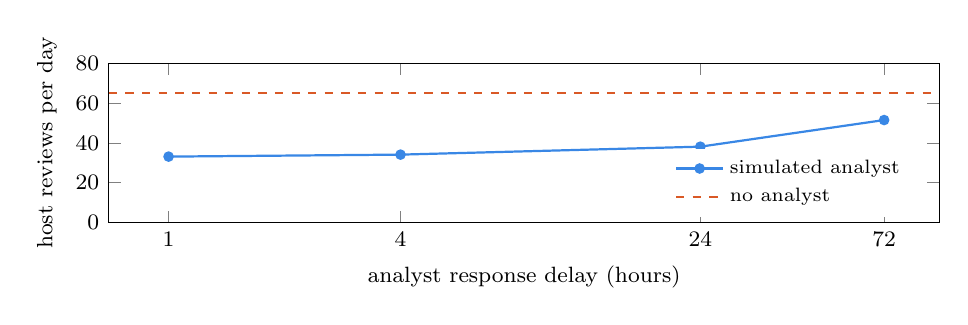
\begin{tikzpicture}
\begin{axis}[width=\columnwidth, height=3.6cm, xmode=log, xmin=0.7, xmax=100, ymin=0, ymax=80,
  xtick=data, log ticks with fixed point, xlabel={analyst response delay (hours)},
  ylabel={host reviews per day}, font=\footnotesize, legend cell align=left, legend pos=south east,
  legend style={font=\scriptsize, draw=none}]
\addplot[cllm, thick, mark=*, mark size=1.5pt] coordinates {(1,33.1) (4,34.1) (24,38.1) (72,51.5)};
\addlegendentry{simulated analyst}
\addplot[ctext, thick, dashed, domain=0.7:100, samples=2] {65.2};
\addlegendentry{no analyst}
\end{axis}
\end{tikzpicture}
\caption{Host reviews per day against the analyst's response delay (targeted unlearning on). At every delay the 72
attack cases were raised and the same 400 attack events alerted.}
\label{fig:delay}
\end{figure}

\subsection{Enforcement Summary}

On the same recorded answers, asymmetric trust left GUIDE suppression unchanged (4/428, 3/437, 10/437), removed
every lost containment, and held E1 at 0/72 dismissals. It raised clean workload from 54.8 to 65.2 reviews per day
without an analyst, and from 33.2 to 34.1 with one, because the model could no longer dismiss. The gpt-oss
containment denominator moved from 176 to 178 for the same reason: two clean pairs whose review request had
cancelled a block under the acting rule.

\section{Discussion and Limitations}\label{sec:disc}

Injected text does steer the model. It hijacked the undefended agent on 29.6\% of pairs, and the steer payload made
NCE name the attacker's chosen host in 30 of 38 cases. What the text achieves depends on the authority the output
carries. With asymmetric trust, the same answers dismissed no attack and cancelled no containment, without the
model having to recognize the attack, as in CaMeL~\cite{camel}. The price is that the LLM, on this data, adds no
measurable value to triage. Asymmetric trust also cannot restore an escalation the model fails to emit when the
model is the only detector (the GUIDE residual).

For memory, the clean-weeks store does most of the work (98.9\% fewer reviews). The gate and D7 kept autonomous
learning from absorbing attacks, but they also kept it from learning anything on host logs: new normal patterns
came only from analysts. The analyst is therefore the remaining poisoning channel. Targeted unlearning closes it for
independent mistakes, but not for host-wide deception.

\emph{Limitations.} (1)~There is one testbed campaign, with labels on two Windows hosts, and the GUIDE pairs are
synthetic. (2)~The analyst and its mistakes are simulated from labels; real fatigue and deception may differ from
our error models, including the persuasion model. (3)~DEDALE uses one model (gpt-oss-20b only on GUIDE development
pairs), and seeds vary the simulated analyst, not the LLM, whose answers were recorded once. (4)~Patterns learned
in the training weeks are permanent, and poisoning during training is out of scope. (5)~NCE sees 512 characters per
field; raw log lines were longer in 718 of 856 cases. (6)~73 of 473 attack events matched learned routine activity;
deliberate mimicry, and escalation flooding against the review queue, were not evaluated. (7)~Statistical power is
low for the small discordant counts, ERA was not ablated on DEDALE, and latency and token cost were not measured.

\section{Conclusion}

GuardedSOC bounds what an LLM and an adaptive store may do in SOC triage. Asymmetric trust made injected log text
unable to dismiss attack cases (0/72) or cancel containment. The quarantined gate kept autonomous learning from
absorbing attacks, and targeted unlearning removed every pattern learned from independent analyst misses. Two
results mark the boundary. Under these rules, the LLM gave no workload reduction over the model-free baseline, and
an analyst persuaded host-wide defeats unlearning. Future work: models that escalate usefully under asymmetric
trust, and defences for the analyst channel.

\section*{Data and Code}

\url{https://github.com/Akshara-reddy612/AgentSOC}: the recorded LLM answers, the scripts that rebuild every number,
the full algorithm, count glossary, pair identifiers and prompts.

\begin{thebibliography}{99}
\bibitem{agentsoc} J.~Roy and S.~K.~Singh, ``AgentSOC: A multi-layer agentic AI framework for security operations
automation,'' in \emph{Proc. 5th IEEE Int. Conf. on AI in Cybersecurity (ICAIC)}, Houston, TX, USA, 2026,
arXiv:2604.20134.
\bibitem{guide} S.~Freitas, J.~Kalajdjieski, A.~Gharib, and R.~McCann, ``AI-driven guided response for security
operation centers with Microsoft Copilot for Security,'' arXiv:2407.09017, 2024.
\bibitem{dedale} M.~Lanvin and F.~Majorczyk, ``DEDALE: Dataset for evaluating detection of APT among logs and
events,'' Recherche Data Gouv, 2026, doi:10.57745/Y5JLDG.
\bibitem{attack} B.~E.~Strom, A.~Applebaum, D.~P.~Miller, K.~C.~Nickels, A.~G.~Pennington, and C.~B.~Thomas,
``MITRE ATT\&CK: Design and philosophy,'' The MITRE Corporation, Tech. Rep., 2018.
\bibitem{alahmadi} B.~A.~Alahmadi, L.~Axon, and I.~Martinovic, ``99\% false positives: A qualitative study of SOC
analysts' perspectives on security alarms,'' in \emph{Proc. 31st USENIX Security Symp.}, 2022.
\bibitem{perez} F.~Perez and I.~Ribeiro, ``Ignore previous prompt: Attack techniques for language models,'' in
\emph{NeurIPS ML Safety Workshop}, 2022, arXiv:2211.09527.
\bibitem{greshake} K.~Greshake, S.~Abdelnabi, S.~Mishra, C.~Endres, T.~Holz, and M.~Fritz, ``Not what you've signed
up for: Compromising real-world LLM-integrated applications with indirect prompt injection,'' in \emph{Proc. 16th
ACM Workshop on Artificial Intelligence and Security (AISec)}, 2023.
\bibitem{liu} Y.~Liu, Y.~Jia, R.~Geng, J.~Jia, and N.~Z.~Gong, ``Formalizing and benchmarking prompt injection
attacks and defenses,'' in \emph{Proc. 33rd USENIX Security Symp.}, 2024.
\bibitem{spotlighting} K.~Hines, G.~Lopez, M.~Hall, F.~Zarfati, Y.~Zunger, and E.~Kiciman, ``Defending against
indirect prompt injection attacks with spotlighting,'' arXiv:2403.14720, 2024.
\bibitem{struq} S.~Chen, J.~Piet, C.~Sitawarin, and D.~Wagner, ``StruQ: Defending against prompt injection with
structured queries,'' in \emph{Proc. 34th USENIX Security Symp.}, 2025.
\bibitem{camel} E.~Debenedetti \emph{et al.}, ``Defeating prompt injections by design,'' arXiv:2503.18813, 2025.
\bibitem{antidote} B.~I.~P.~Rubinstein, B.~Nelson, L.~Huang, A.~D.~Joseph, S.~Lau, S.~Rao, N.~Taft, and
J.~D.~Tygar, ``ANTIDOTE: Understanding and defending against poisoning of anomaly detectors,'' in \emph{Proc. 9th
ACM SIGCOMM Internet Measurement Conf. (IMC)}, 2009.
\bibitem{agentpoison} Z.~Chen, Z.~Xiang, C.~Xiao, D.~Song, and B.~Li, ``AgentPoison: Red-teaming LLM agents via
poisoning memory or knowledge bases,'' in \emph{Advances in Neural Information Processing Systems (NeurIPS)}, 2024.
\bibitem{poisonedrag} W.~Zou, R.~Geng, B.~Wang, and J.~Jia, ``PoisonedRAG: Knowledge corruption attacks to
retrieval-augmented generation of large language models,'' in \emph{Proc. 34th USENIX Security Symp.}, 2025.
\bibitem{unlearning} Y.~Cao and J.~Yang, ``Towards making systems forget with machine unlearning,'' in \emph{Proc.
IEEE Symp. on Security and Privacy (S\&P)}, 2015.
\bibitem{hierarchy} E.~Wallace, K.~Xiao, R.~Leike, L.~Weng, J.~Heidecke, and A.~Beutel, ``The instruction
hierarchy: Training LLMs to prioritize privileged instructions,'' arXiv:2404.13208, 2024.
\bibitem{agentdojo} E.~Debenedetti, J.~Zhang, M.~Balunovi\'{c}, L.~Beurer-Kellner, M.~Fischer, and F.~Tram\`{e}r,
``AgentDojo: A dynamic environment to evaluate prompt injection attacks and defenses for LLM agents,''
arXiv:2406.13352, 2024.
\bibitem{injecagent} Q.~Zhan, Z.~Liang, Z.~Ying, and D.~Kang, ``InjecAgent: Benchmarking indirect prompt injections
in tool-integrated large language model agents,'' arXiv:2403.02691, 2024.
\bibitem{memorypoison} P.~Dash, T.~Ge, A.~Jain, T.~Shah, and Z.~Shang, ``From untrusted input to trusted memory: A
systematic study of memory poisoning attacks in LLM agents,'' arXiv:2606.04329, 2026.
\bibitem{memstream} S.~Bhatia, A.~Jain, S.~Srivastava, K.~Kawaguchi, and B.~Hooi, ``MemStream: Memory-based
streaming anomaly detection,'' arXiv:2106.03837, 2021.
\bibitem{tsegai} S.~A.~Tsegai, A.~Kantchelian, D.~Yao, and P.~Gao, ``From investigation failures to reliable SOC
agents: Understanding and improving LLM-based alert triage,'' arXiv:2610.10608, 2026.
\end{thebibliography}

\end{document}
